\graphicspath{{./}{./fig/}{./fig/cachebar/}}
\chapter[\uppercase{A defense against cache-based
side channels with empirical security}]{\uppercase{A defense against cache-based
side channels with empirical security}\protect\footnote{This chapter is excerpted from previously
published work~\cite{cachebar} coauthored with Michael K. Reiter and
Yinqian Zhang.}}
\label{chap:cachebar}
This chapter focuses on information leakage through the cache-based
side channels in \glspl{LLC}. We expect to use this dedicated example
to emphasize the importance of measuring with static analysis, by
comparing the empirical measure and static verification based on a
formal model.

Recall that \flushreload, \primeprobe,
and their variants are the most commonly used attack vectors in
cache-based side channels. We propose a software-only defense against
these \gls{LLC}-based side-channel attacks, based on two seemingly
straightforward principles. First, to defeat \flushreload attacks, we
propose a \coa mechanism to manage physical pages shared across
mutually distrusting \textit{security domains} (i.e., processes,
containers\footnote{https://linuxcontainers.org/}, or \glspl{VM}).
Specifically, temporally proximate accesses to the same physical page
by multiple security domains results in the page being copied so that
each domain has its own copy.  In this way, a victim's access to its
copy will be invisible to an attacker's \Reload in a \flushreload
attack. When accesses are sufficiently spaced in time, the copies can
be deduplicated to return the overall memory footprint to its original
size. Second, to defeat \primeprobe attacks, we design a mechanism to
manage the cacheability of memory pages so as to limit the number of
lines per cache set that an attacker may \Probe. In doing so, we limit
the attacker's visibility into the victim's demand for memory that
maps to that cache set.  

Of course, the essential part of defense work is to prove their
effectiveness through a reasonable security evaluation. To do so, we
first detail design and implementation in a memory management
subsystem called \cachebar (short for ``\cachebarLong'') for the Linux
kernel.  \cachebar supports these defenses for security domains
represented as Linux containers.  That is, \coa to defend against
\flushreload attacks makes page copies as needed to isolate temporally
proximate accesses to the same page from different containers.
Moreover, memory cacheability is managed so that the processes in each
container are collectively limited in the number of lines per cache
set they can \Probe. \cachebar would thus be well-suited for use in
\gls{PaaS} clouds that isolate cloud customers in distinct containers.
With a concrete implementation, we design a quantitative empirical
evaluation to measure the attacker's ability to distinguish a victim's
behavior in a \gls{PaaS} cloud environment. Our empirical results show
that \cachebar effectively restricts the leakage in cache-based
side-channel attacks. Besides, we build a formal model for \coa and
use model checking to check potential interference. The checking
results reveal the incompleteness of empirical evaluation, which
covers more vulnerable information flows than rerunning concrete
attacks. 

\section{Copy-On-Access}
\label{cachebar:sec:coa}
\subsection{Design}
\label{cachebar:sec:coa:design}

Modern operating systems, in particular Linux \gls{OS}, often adopt
on-demand paging and copy-on-write mechanisms to
reduce the memory footprints of userspace applications. In particular,
copy-on-write enables multiple processes to share the same set of
physical memory pages as long as none of them modify the content.  If
a process writes to a shared memory page, the write will trigger a
page fault and a subsequent new page allocation so that a private copy
of page will be provided to this process. In addition, memory merging
techniques like \KSM~\cite{arcangeli2009increasing} are also used in
Linux \gls{OS} to deduplicate identical memory pages.  Memory sharing,
however, is one of the key factors that enable \flushreload
side-channel attacks.  Disabling memory page sharing entirely will
eliminate \flushreload side channels but at the cost of much larger
memory footprints and thus inefficient use of physical memory.

\begin{figure}%
%\vspace{-2ex}
\centering
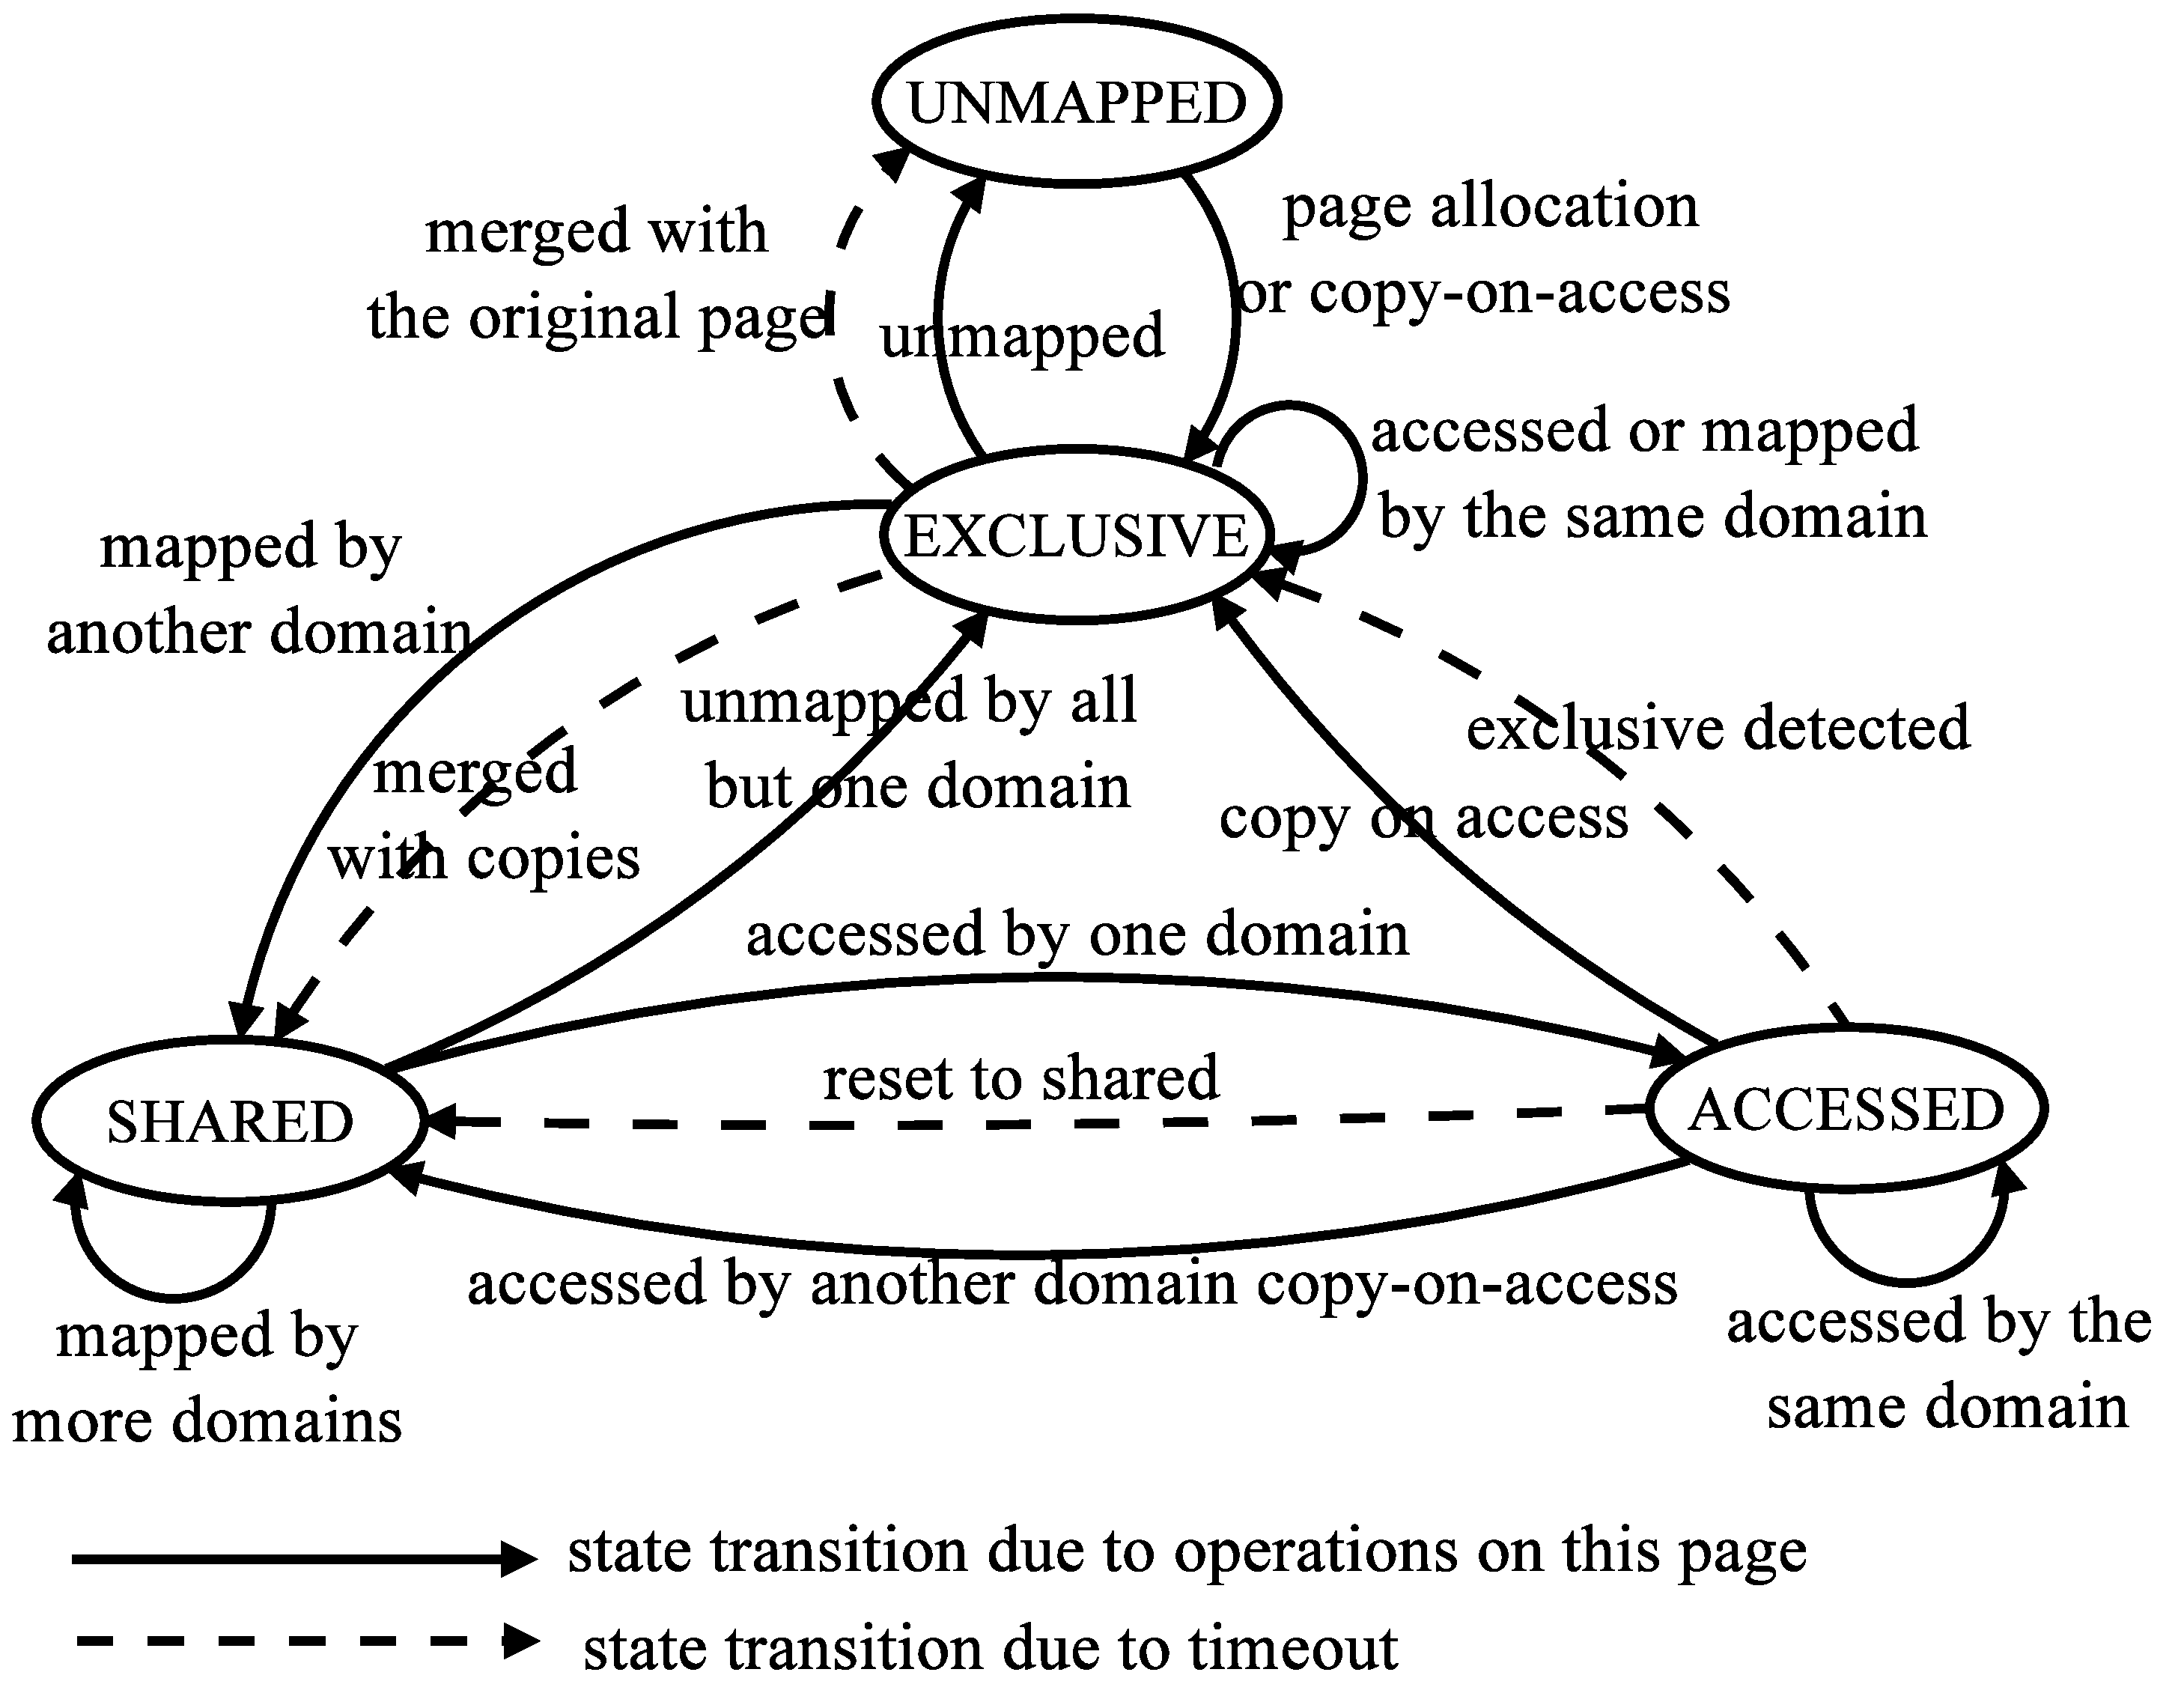
\includegraphics[width=0.7\linewidth]{fig/cachebar/states.eps}
%\resizebox{\linewidth}{!}{\large\input{fig/cachebar/states.eps}}%
\caption{Copy-On-Access State Transition\label{fig:coa}}%
\end{figure}

\cachebar adopts a design that we call \coa, which dynamically controls
the sharing of physical memory pages between security domains. We
designate each physical page as being in exactly one of the following
states: \unmapped, \exclusive, \shared, and \accessed.  An \unmapped
page is a physical page that is not currently in use. An \exclusive
page is a physical page that is currently used by exactly one security
domain, but may be shared by multiple processes in that domain.
A \shared page is a physical page that is shared by multiple security
domains, i.e., mapped by at least one process of each of the sharing
domains, but no process in any domain has accessed this physical page
recently. In contrast, an \accessed page is a previously \shared page
that was recently accessed by a security domain.  The state
transitions are shown in \figref{fig:coa}.

An \unmapped page can transition to the \exclusive state either due to
normal page mapping, or due to copy-on-access when a page is copied
into it.  Unmapping a physical page for any reason (e.g., process
termination, page swapping) will move an \exclusive page back to the
\unmapped state. However, mapping the current \exclusive page by
another security domain will transit it into the \shared state.  If
all but one domain unmaps this page, it will transition back from the
\shared state to the \exclusive state, or \accessed state to the
\exclusive state.  A page in the \shared state may be shared by more
domains and remain in the same state; when any one of the domains
accesses the page, it will transition to the \accessed state. An
\accessed page can stay that way as long only the same security domain
accesses it.  If this page is accessed by another domain, a new
physical page will be allocated to make a copy of this one, and the
current page will transition to either \exclusive or \shared state,
depending on the remaining number of domains mapping this page. The
new page will be assigned state \exclusive.  An \accessed page will be
reset to the \shared state if it is not accessed for \accessedTimeout
seconds. This timeout mechanism ensures that only recently used pages
will remain in the \accessed state, limiting chances for unnecessary
duplication.
Page merging may also be triggered by deduplication services in a
modern \gls{OS} (e.g., \gls{KSM} in Linux).  This effect is reflected by a dashed
line in \figref{fig:coa} from state \exclusive to \shared.  A page
at any of the \textit{mapped} states (i.e., \exclusive, \shared,
\accessed) can transition to \unmapped state for the same reason when
it is a copy of another page (not shown in the figure).

Merging duplicated pages requires some extra bookkeeping. When
a page transitions from \unmapped to \exclusive due to copy-on-access,
the original page is tracked by the new copy so that \cachebar knows
with which page to merge it when deduplicating.  If
the original page is unmapped first, then one of its
copies will be designated as the new ``original''
page, with which other copies will be merged in the future. The interaction between copy-on-access
and existing copy-on-write mechanisms is also implicitly depicted in
\figref{fig:coa}: Upon copy-on-write, the triggering process will first
\textit{unmap} the physical page, possibly inducing a state transition (from
\shared to \exclusive). The state of the newly mapped physical page is
maintained separately.

\subsection{Implementation}
\label{cachebar:sec:coa:impl}

At the core of copy-on-access implementation is the state machine depicted in
\figref{fig:coa}.

\bheading{\unmapped $\Leftrightarrow$ \exclusive
  $\Leftrightarrow$ \shared}
Conventional Linux kernels maintain the relationship between processes
and the physical pages they use.  However, \cachebar also needs to keep
track of the relationship between containers and the physical pages
that each container's processes use.  Therefore, \cachebar incorporates
a new data structure, \pcounterincontainer, which is conceptually a
table used for recording, for each physical page, the number of
processes in each container that have \glspl{PTE} mapped
to this page. 

The \pcounterincontainer data structure is updated and referenced in
multiple places in the kernel.  Specifically, in \cachebar we
instrumented every update of \mapcount, a data field in the
\texttt{page} structure for counting \gls{PTE} mappings, so that every time
the kernel tracks the \gls{PTE} mappings of a physical page,
\pcounterincontainer is updated accordingly. The use of
\pcounterincontainer greatly simplifies maintaining and determining
the state of a physical page: (1) Given a container, access to a
single cell suffices to check whether a physical page is already
mapped in the container. This operation is very commonly used to
decide if a state transition is required when a page is mapped by a
process.  Without \pcounterincontainer, such an operation requires
performing reverse mappings to check the domain of each mapping. (2)
Given a physical page, it takes \containerNmbr accesses to
\pcounterincontainer, where \containerNmbr is the total number of
containers, to tell which containers have mapped to this
page. This operation is commonly used to determine the state of a
physical page.

\bheading{\shared $\Rightarrow$ \accessed}
\begin{figure}[tb]
\centering
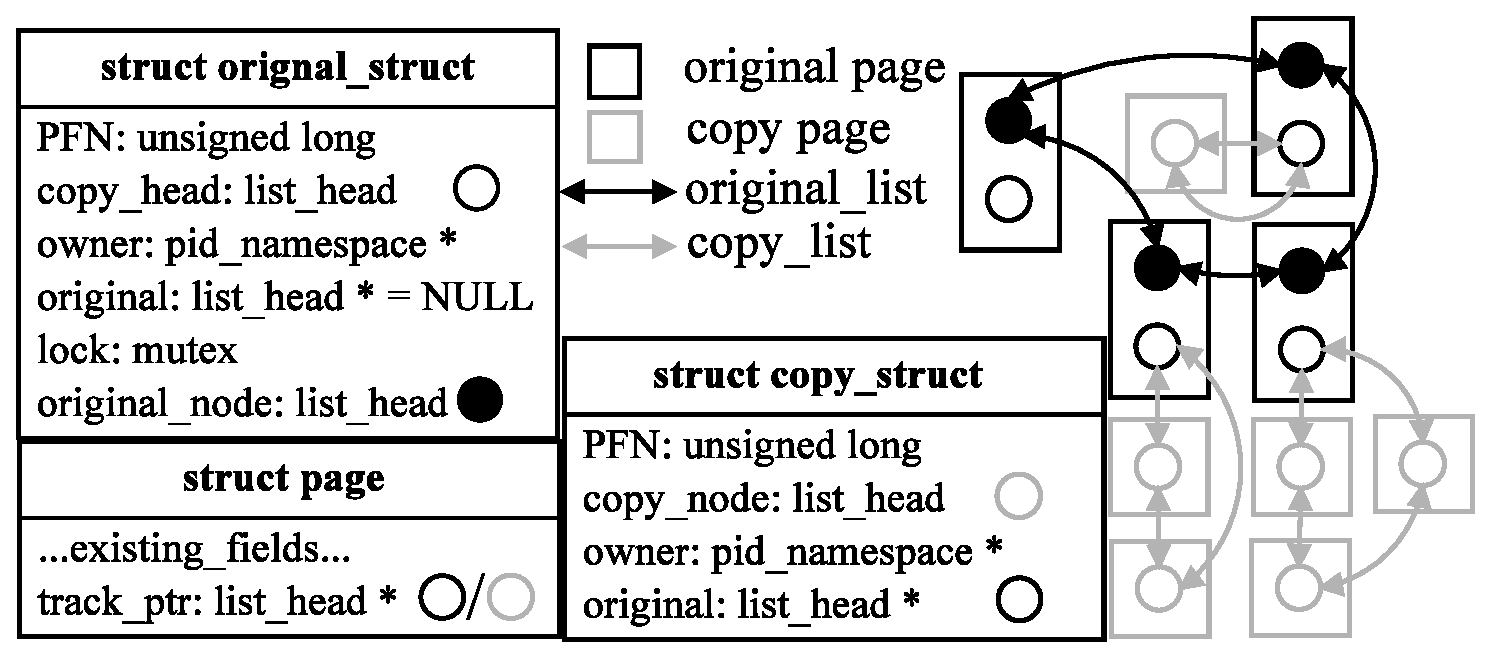
\includegraphics[width=0.7\linewidth]{fig/cachebar/coa_struct.eps}
\caption{Structure of \coa page lists.}
\label{fig:linkedlist}
\end{figure} 
To differentiate \shared and \accessed states, one additional data field,
\owner, is added (see \figref{fig:linkedlist}) to indicate the owner of the page
(a pointer to a \texttt{PID\_namespace} structure). When the page is in the
\shared state, its \owner is \texttt{NULL}; otherwise it points to the
container that last accessed it.

All \gls{PTE}s pointing to a \shared physical page will have a reserved \COA
bit set. Therefore, any access to these virtual pages will induce a
page fault.  When a page fault is triggered, \cachebar checks if the
page is present in physical memory; if so, and if the physical page is
in the \shared state, the \COA bit of the current \gls{PTE} for this page
will be cleared so that additional accesses to this physical page from
the current process will be allowed without page faults.  The physical
page will also transition to the \accessed state.

\bheading{\accessed $\Rightarrow$ \exclusive/\shared}  If the page is
already in the \accessed state when a domain other than the \owner
accesses it, the page fault handler will allocate a new physical page,
copy the content of the original page into the new page, and change
the \gls{PTE}s in the accessing container so that they
point to the new page. Since multiple same-content copies in one
domain burdens both performance and memory but contributes nothing for
security, the fault handler will reuse a copy belonging to that domain
if it exists. After copy-on-access, the original page can either be
\exclusive or \shared.  All copy pages are anonymous-mapped, since
only a single file-mapped page for the same file section is allowed.

A transition from the \accessed state to \shared or \exclusive state
can also be triggered by a timeout mechanism. \cachebar implements a
periodic timer (every $\accessedTimeout = 1\secs$). Upon timer
expiration, all physical pages in the \accessed state that were
not accessed during this \accessedTimeout interval will be reset to
the \shared state by clearing its \owner field, so that pages that are
infrequently accessed are less likely to trigger \coa.  If an
\accessed page is found for which its \pcounterincontainer shows the
number of domains mapped to it is 1, then the daemon instead clears
the \COA bit of all \gls{PTE}s for that page and marks the page \exclusive.

Instead of keeping a list of \accessed pages, \cachebar maintains a
list of pages that are in either \shared or \accessed state, denoted
\originalpagelist (shown in \figref{fig:linkedlist}). Each node in the
list also maintains a list of copies of the page it represents, dubbed
\copypagelist. These lists are attached onto the \texttt{struct page}
through \texttt{track\_ptr}.  Whenever a copy is made from the page
upon \coa, it is inserted into the \copypagelist of the original page.
Whenever a physical page transitions to the \unmapped state, it is
removed from whichever of \originalpagelist or \copypagelist it is
contained in.  In the former case, \cachebar will designate a copy
page of the original page as the new original page and adjust the
lists accordingly.

For security reasons that will be explained in
\secref{cachebar:sec:coa:security}, we further require flushing the entire
memory page out of the cache after transitioning a page from the
\accessed state to the \shared state due to this timeout
mechanism. This page-flushing procedure is implemented by issuing
\texttt{clflush} on each of the memory blocks of any virtual page that
maps to this physical page.

\bheading{State transition upon \clflush} The \clflush instruction is
subject to the same permission checks as a memory load, will trigger
the same page faults,
and will similarly set the ACCESSED bit in the \gls{PTE} of its
argument~\cite{guide2010intel}.  As such, each \Flush via \clflush
triggers the same transitions (e.g., from \shared to \accessed, and
from \accessed to an \exclusive copy) as a \Reload in our
implementation, meaning that this defense is equally effective against
both \flushreload and \flushflush~\cite{gruss:2015:FF} attacks.

\bheading{Page deduplication}  To mitigate the impact of \coa on the
size of memory, \cachebar implements a less frequent timer (every
$\copyTimeout = 10\times\accessedTimeout$ seconds) to periodically
merge the page copies with their original pages. Within the timer
interrupt handler, \originalpagelist and each \copypagelist are
traversed similarly to the ``\accessed $\Rightarrow$ \shared''
transition description above, though the ACCESSED bit in the \gls{PTE}s of
only pages that are in the \exclusive state are checked. If a copy
page has not been accessed since the last such check (i.e., the
ACCESSED bit is unset in all \gls{PTE}s pointing to it), it will be merged
with its original page (the head of the \copypagelist). The ACCESSED
bit in the \gls{PTE}s will be cleared afterwards.

When merging two pages, if the original page is anonymous-mapped, then
the copy page can be merged by simply updating all \gls{PTE}s pointing to
the copy page to instead point to the original page, and then updating
the original page's reverse mappings to include these \gls{PTE}s.  If the
original page is file-mapped, then merging is more
intricate, additionally involving the creation of a new virtual memory
area (\texttt{vma} structure) that maps to the original page's file
position and using this structure to replace the virtual memory area
of the (anonymous) copy page in the relevant task structure.

For security reasons, merging of two pages requires flushing the
original physical page from the \gls{LLC}.  We will elaborate on this point
in \secref{cachebar:sec:coa:security}.

\bheading{Interacting with \gls{KSM}}  
Page deduplication can also be triggered by existing memory
deduplication mechanisms (e.g., \gls{KSM}). To maintain the state of
physical pages, \cachebar instruments every reference to \mapcount
within \gls{KSM} and updates \pcounterincontainer accordingly.
\gls{KSM} is capable of merging more pages than our built-in page
deduplication mechanisms.  However, \cachebar still relies on the built-in page
deduplication mechanisms for several reasons. First, \gls{KSM} can merge only
anonymous-mapped pages, while \cachebar needs to frequently merge an
anonymous-mapped page (a copy) with a file-mapped page (the original). Second,
\gls{KSM} may not be enabled in certain settings, which will lead to ever growing
\copypagelist{s}.  Third, \gls{KSM} must compare page contents byte-by-byte before
merging two pages, whereas \cachebar deduplicates pages on the
same \copypagelist, avoiding the expensive page content comparison.


\section{Cacheability Management}
\label{cachebar:sec:cacheabilityMgmt}

A potentially effective countermeasure to \primeprobe attacks is to
remove the attacker's ability to \Prime and \Probe the whole cache set
and to predict how a victim's demand for that set will be reflected in
the number of evictions from that set.

\subsection{Design}
\label{cachebar:sec:cacheabilityMgmt:design}
\begin{figure}[t]
\centering
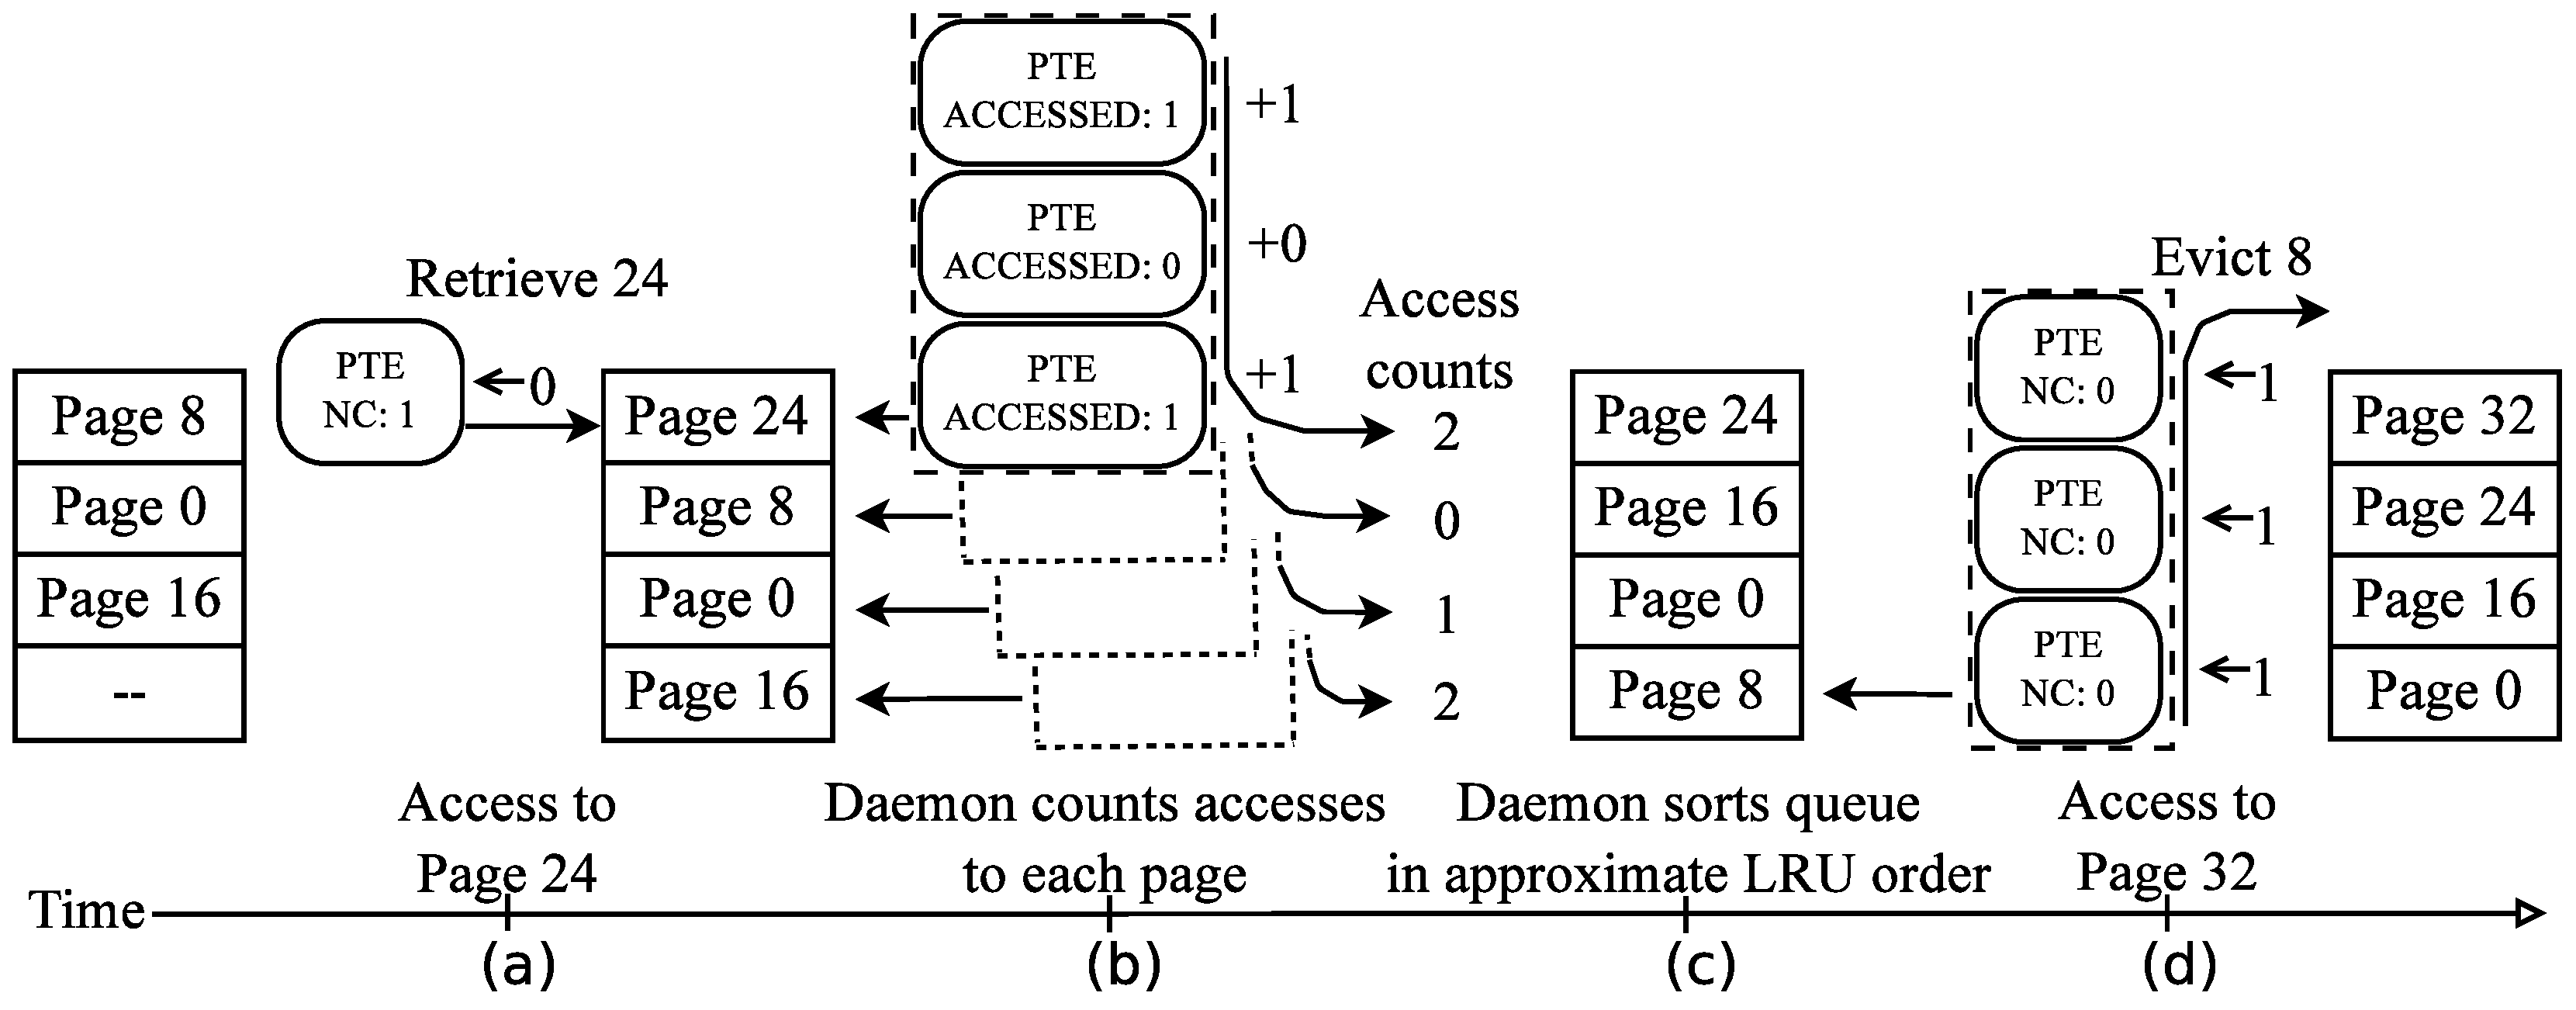
\includegraphics[width=0.85\textwidth]{fig/cachebar/queue-all.eps}
\caption[A \lru for one page color in a domain]{A \lru for one page color in a domain: (a) access to page 24
brings it into the queue and clears NC bit (``$\leftarrow\!0$'') in
the PTE triggering the fault; periodically, (b) a daemon counts
the ACCESSED bits (``$+0$'', ``$+1$'') per page and (c) reorders pages
accordingly; to make room for a new page, (d) NC bits in PTE
pointing to the least recently used page are set, and the page is
removed from the queue.}
\label{fig:queues:all}
\vspace{-0.1in}
\end{figure}
Suppose a \cacheLineNmbr-way set associative \gls{LLC}, so that each
cache set has \cacheLineNmbr lines.  Let \evictedNmbr be the number of
cache lines in one set that the attacker observes having been evicted
in a \primeprobe interval (i.e., $\evictedNmbr \in \AOOKeys{}$).  The
\primeprobe attack is effective today because \evictedNmbr is
typically a good indicator of the demand \victimDemand that the victim
security domain had for memory that mapped to that cache set during
the \primeprobe interval (i.e., $\victimDemand\in \SecKeys{}$).  In
particular, if the attacker \Prime{s} and \Probe{s} all \cacheLineNmbr
lines, then it can often observe the victim's demand \victimDemand
exactly, unless $\victimDemand > \cacheLineNmbr$ (in which case the
attacker learns at least $\victimDemand \ge \cacheLineNmbr$).

Here we propose to periodically and
probabilistically reconfigure the budget
\linesPerContainer{\containerIdx} of lines per cache set that the
security domain \containerIdx can occupy.  After such a
reconfiguration, the attacker's view of the victim's demand
\victimDemand is clouded by the following three effects.  First, if
the attacker is allotted a budget $\linesPerContainer{\attackerLabel}
< \cacheLineNmbr$, then the attacker will be unable to observe any
evictions at all (i.e., $\evictedNmbr=0$) if $\victimDemand <
\cacheLineNmbr-\linesPerContainer{\attackerLabel}$.\footnote{This
  statement assumes a LRU replacement policy and that
  the victim is the only security domain that runs in the \primeprobe
  interval.  If it was not the only security domain to run, then the ambiguity of 
  the observable evictions will additionally cause difficulties for
  the attacker.}  Second, if the victim is given allotment
\linesPerContainer{\victimLabel}, then any two victim demands
\victimDemand, \victimDemandAlt satisfying $\victimDemand >
\victimDemandAlt \ge \linesPerContainer{\victimLabel}$ will be
indistinguishable to the attacker.  Third, the probabilistic
assignment of \linesPerContainer{\victimLabel} results in extra
ambiguity for the attacker, since \evictedNmbr evictions might reflect
the demand \victimDemand or the budget
\linesPerContainer{\victimLabel}, since $\evictedNmbr \le
\min\{\victimDemand,\linesPerContainer{\victimLabel}\}$ (if all
\evictedNmbr evictions are caused by the victim).

To enforce the budget \linesPerContainer{\containerIdx} of lines that
security domain \containerIdx can use in a given cache set, \cachebar
maintains for each cache set a queue per security domain that records
which memory blocks are presently cacheable in this set by processes
in this domain.  Each element in the queue indicates a memory block
that maps to this cache set; only blocks listed in the queue can be
cached in that set.  The queue is maintained with a least recently
used (LRU) replacement algorithm. That is, whenever a new memory block
is accessed, it will replace the memory block in the corresponding
queue that is the least recently used.

\subsection{Dynamic budget \linesPerContainer{\containerIdx} of
cache lines}
\label{cachebar:sec:cacheabilityMgmt:security}
\if0
While the budget \linesPerContainer{\containerIdx} is in effect, each
access to a memory block that maps to this cache set, beyond the
in-queue \linesPerContainer{\containerIdx} memory blocks, will incur a
page fault (because they are all in different pages).  Because the
page-fault processing time will overwhelm the timing granularity of
modern \primeprobe attacks by an order of magnitude, the attacker
\containerIdx realistically needs to restrict himself to accessing
\linesPerContainer{\containerIdx} pages in his \Probe phase and hence
to occupying \linesPerContainer{\containerIdx} lines in that cache
set. The security of this design hinges critically on how each
\linesPerContainer{\containerIdx} is set by the daemon.  When
\linesPerContainer{\containerIdx} is reset, it is drawn from a
distribution.  In the remainder of this section we present how this
distribution is determined.
\fi

Suppose there are (at most) \attackerNmbr domains on a host that are
owned by the attacker---which might be all  domains on the host except
the victim---and let \cacheLineNmbr be the number of cache lines per
\gls{LLC} set. Below we consider domain $0$ to be the ``victim''
domain being subjected to \primeprobe attacks by the ``attacker''
domains $1, \ldots, \attackerNmbr$.  Of course, the attacker domains
make use of all $\sum_{\containerIdx=1}^{\attackerNmbr}
\linesPerContainer{\containerIdx}$ cache lines available to them for
conducting their \primeprobe attacks.

Periodically, \cachebar draws a new value
\linesPerContainer{\containerIdx} for each security domain
\containerIdx.  This drawing is memoryless and independent of the
draws for other security domains.  Let
\linesPerContainerRV{\containerIdx} denote the random variable
distributed according to how \linesPerContainer{\containerIdx} is
determined.  The random variables that we presume can be observed by
the attacker domains include $\linesPerContainerRV{1}, \ldots,
\linesPerContainerRV{\attackerNmbr}$; let $\attackerLineNmbrRV{}\!=
\!\min\left\{\cacheLineNmbr, \sum_{\containerIdx=1}^{\attackerNmbr}
\linesPerContainerRV{\containerIdx}\right\}$ denote the number of
cache lines allocated to the attacker domains.  We also presume the
attacker can accurately measure the number \evictedNmbrRV of its cache
lines that are evicted during the victim's execution.

Let \prob{\victimDemand}{\genericEvent} denote the probability of
event \genericEvent in an execution period during which the victim's
cache usage would populate \victimDemand lines (of this color) if it
were allowed to use all \cacheLineNmbr lines, i.e., if
$\linesPerContainer{0} = \cacheLineNmbr$.  We (the defender) would
like to distribute $\linesPerContainerRV{0}, \ldots,
\linesPerContainerRV{\attackerNmbr}$
so as to minimize the statistical distance between eviction
distributions observable by the attacker for different victim demands
\victimDemand, \victimDemandAlt, i.e., to minimize
\begin{align}
\sum_{0 \le \victimDemand < \victimDemandAlt \le \cacheLineNmbr} \sum_{\evictedNmbr} |\prob{\victimDemand}{\evictedNmbrRV = \evictedNmbr} - \prob{\victimDemandAlt}{\evictedNmbrRV = \evictedNmbr}|
\label{eqn:securityGoal}
\end{align}

We begin by deriving an expression
for \prob{\victimDemand}{\evictedNmbrRV = \evictedNmbr}.  Below we
make the conservative assumption that all evictions are caused by the
victim's behavior; in reality, caches are far noisier.  We first
consider the case $\evictedNmbr=0$, i.e., that the attacker domains
observe no evictions.
\begin{align*}
\cprob{\Big}{\victimDemand}{\evictedNmbrRV =
0}{\linesPerContainerRV{0} = \linesPerContainer{0}
\wedge~\attackerLineNmbrRV =
\attackerLineNmbr}
& \!=\! \left\{\begin{array}{@{\extracolsep{-0.4em}}ll}
1 & \mbox{if $\cacheLineNmbr \ge \attackerLineNmbr + \min\{\linesPerContainer{0}, \victimDemand\}$} \\
0 & \mbox{otherwise}
\end{array}\right.
\end{align*}
``$\min\{\linesPerContainer{0}, \victimDemand\}$'' is used above
because any victim demand for memory blocks that map to this cache set
beyond \linesPerContainer{0} will back-fill the cache lines invalidated
when \cachebar flushes other blocks from the victim's cacheability
queue, rather than evicting others.  Since \linesPerContainerRV{0} and
\attackerLineNmbrRV are independent,
\begin{align}
\prob{\victimDemand}{\evictedNmbrRV = 0}
& = \sum_{\linesPerContainer{0}=0}^{\victimDemand}
\sum_{\attackerLineNmbr=0}^{\cacheLineNmbr-\linesPerContainer{0}}
\prob{}{\linesPerContainerRV{0} = \linesPerContainer{0}} \cdot
\prob{}{\attackerLineNmbrRV = \attackerLineNmbr}
 + \sum_{\linesPerContainer{0}=\victimDemand+1}^{\cacheLineNmbr} \sum_{\attackerLineNmbr=0}^{\cacheLineNmbr-\victimDemand} \prob{}{\linesPerContainerRV{0} = \linesPerContainer{0}} \cdot \prob{}{\attackerLineNmbrRV = \attackerLineNmbr} \label{eqn:zeroEvictions}
\end{align}
Note that we have dropped the ``\victimDemand'' subscripts from the
probabilities on the right, since \linesPerContainerRV{0}
and \attackerLineNmbrRV are distributed independently
of \victimDemand.  And, since
$\linesPerContainerRV{1},\ldots,\linesPerContainerRV{\attackerNmbr}$
are independent,
\begin{align}
\prob{}{\attackerLineNmbrRV\!=\!\attackerLineNmbr} = \!\begin{cases}
\displaystyle
\sum_{ \linesPerContainer{1}\!+\ldots+\!\linesPerContainer{\attackerNmbr}=\attackerLineNmbr} \prod_{\containerIdx=1}^{\attackerNmbr} \prob{}{\linesPerContainerRV{\containerIdx} = \linesPerContainer{\containerIdx}} & \mbox{if $\attackerLineNmbr\!<\!\cacheLineNmbr$}\\
\displaystyle
\sum_{\linesPerContainer{1}\!+\ldots+\!\linesPerContainer{\attackerNmbr}\ge\cacheLineNmbr} \prod_{\containerIdx=1}^{\attackerNmbr} \prob{}{\linesPerContainerRV{\containerIdx} = \linesPerContainer{\containerIdx}} & \mbox{if $\attackerLineNmbr\!=\!\cacheLineNmbr$}
\end{cases}
\label{eqn:attackerLineNmbr}
\end{align}

Similarly, for $\evictedNmbr \ge 1$, 
\begin{align*}
\cprob{\Big}{\victimDemand}{\evictedNmbrRV=\evictedNmbr}{\linesPerContainerRV{0} = \linesPerContainer{0} \wedge\attackerLineNmbrRV = \attackerLineNmbr}
& = \left\{\begin{array}{ll}
1 & \mbox{if $\evictedNmbr\! +\!\cacheLineNmbr = \attackerLineNmbr\! + \!\min\{\linesPerContainer{0}, \victimDemand\}$} \\
0 & \mbox{otherwise}
\end{array}\right.
\end{align*}
and so for $\evictedNmbr \ge 1$,
\begin{align}
\prob{\victimDemand}{\evictedNmbrRV = \evictedNmbr}
& = \sum_{\linesPerContainer{0}=0}^{\victimDemand} \prob{}{\linesPerContainerRV{0} = \linesPerContainer{0}} \cdot \prob{}{\attackerLineNmbrRV = \evictedNmbr\! +\! \cacheLineNmbr \!-\! \linesPerContainer{0}} 
+\sum_{\linesPerContainer{0}=\victimDemand+1}^{\cacheLineNmbr} \hspace{-0.53em}\prob{}{\linesPerContainerRV{0} = \linesPerContainer{0}} \cdot \prob{}{\attackerLineNmbrRV = \evictedNmbr\! +\! \cacheLineNmbr \!-\! \victimDemand}
\label{eqn:moreThanZeroEvictions}
\end{align}

From here, we proceed to solve for the best distribution for
$\linesPerContainerRV{0}, \ldots, \linesPerContainerRV{\attackerNmbr}$
to minimize \eqnref{eqn:securityGoal} subject to
constraints \eqnsref{eqn:zeroEvictions}{eqn:moreThanZeroEvictions}.
That is, we specify
those constraints, along with
\begin{align}
\forall \containerIdx, \containerIdxAlt, \linesPerContainer{}:~ &
\prob{}{\linesPerContainerRV{\containerIdx} = \linesPerContainer{}} = \prob{}{\linesPerContainerRV{\containerIdxAlt} = \linesPerContainer{}} \label{eqn:allDistsSame}\\
\forall \containerIdx:~ &
\sum_{\linesPerContainer{\containerIdx} = 0}^{\cacheLineNmbr} \prob{}{\linesPerContainerRV{\containerIdx} = \linesPerContainer{\containerIdx}} = 1 \\
\forall \containerIdx, \linesPerContainer{\containerIdx}:~ &
\prob{}{\linesPerContainerRV{\containerIdx} = \linesPerContainer{\containerIdx}} \ge 0 \label{eqn:nonnegProbs}
\end{align}
and then solve for each \prob{}{\linesPerContainerRV{\containerIdx}
= \linesPerContainer{\containerIdx}} to
minimize \eqnref{eqn:securityGoal}.

Unfortunately, solving to minimize \eqnref{eqn:securityGoal} alone
simply results in a distribution that results in no use of the cache
at all (e.g., $\prob{}{\linesPerContainerRV{\containerIdx}=0} = 1$ for
each \containerIdx).  As such, we need to rule out such degenerate
and ``unfair'' cases:
\begin{align}
\forall \containerIdx:~ &
\prob{}{\linesPerContainerRV{\containerIdx}
        < \cacheLineNmbr/(\attackerNmbr+1)} = 0
\label{eqn:fairness}
\end{align}
Also, to encourage cache usage, we counterbalance
\eqnref{eqn:securityGoal} with a second goal that
values greater use of the cache.  We express this goal as minimizing
the earth mover's distance~\cite{elizaveta2001emd} from
the distribution that assigns
$\prob{}{\linesPerContainerRV{\containerIdx} = \cacheLineNmbr} = 1$,
i.e.,
\begin{align}
\sum_{\linesPerContainer{}=0}^{\cacheLineNmbr} (\cacheLineNmbr-\linesPerContainer{})
\cdot \prob{}{\linesPerContainerRV{0} = \linesPerContainer{}}
\label{eqn:performanceGoal}
\end{align}

As such, the final optimization problem seeks to balance
\eqnref{eqn:securityGoal} and \eqnref{eqn:performanceGoal}.  Let
constant \maxSecValue denote the maximum (i.e., worst) possible value
of \eqnref{eqn:securityGoal} (i.e., when
$\prob{}{\linesPerContainerRV{\containerIdx}=\cacheLineNmbr} = 1$ for
each \containerIdx) and \maxPerfValue denote the maximum (i.e., worst)
possible value of \eqnref{eqn:performanceGoal} (i.e., when
$\prob{}{\linesPerContainerRV{\containerIdx}=0} = 1$ for
each \containerIdx).  Then, given a parameter \balanceSlack, $0
< \balanceSlack < 1$, our optimization computes
distributions
for $\linesPerContainerRV{0}, \ldots, \linesPerContainerRV{\attackerNmbr}$
so as to minimize \balanceValue subject to
\vspace{-5pt}
\begin{align*}
\balanceValue & = \frac{1}{\maxSecValue} \left(\sum_{0 \le \victimDemand < \victimDemandAlt \le \cacheLineNmbr} \sum_{\evictedNmbr} |\prob{\victimDemand}{\evictedNmbrRV = \evictedNmbr} - \prob{\victimDemandAlt}{\evictedNmbrRV = \evictedNmbr}|\right) \\
\balanceValue & \ge \frac{1}{\maxPerfValue(1+\balanceSlack)} \left(\sum_{\linesPerContainer{}=0}^{\cacheLineNmbr} (\cacheLineNmbr-\linesPerContainer{})
\cdot \prob{}{\linesPerContainerRV{0} = \linesPerContainer{}}\right)
\end{align*}
and constraints \eqnsref{eqn:zeroEvictions}{eqn:fairness}.

The evaluation in \secref{cachebar:sec:eval:security:primeprobe}
empirically characterizes the security that result from setting
$\balanceSlack = 0.01$ the default setting in \cachebar.  

\subsection{Implementation}
\label{cachebar:sec:cacheabilityMgmt:impl}

Implementation of \lru{s} is processor micro-architecture dependent.
Here we focus our attention on Intel x86 processors, which appears to
be more vulnerable to \primeprobe attacks due to their inclusive
last-level cache~\cite{liu2015practical}.  As x86 architectures only
support memory management at the page granularity (e.g., by
manipulating the \gls{PTE}s to cause page faults), \cachebar controls the
cacheability of memory blocks at page granularity.  \cachebar uses
reserved bits in each \gls{PTE} to manage the cacheability of, and to track
accesses to, the physical page to which it points, since a reserved
bit set in a \gls{PTE} induces a page fault upon access to the associated
virtual page, for which the backing physical page cannot be retrieved
or cached (if it is not already) before the bit is
cleared~\cite{guide2010intel,raikin2014tracking}.  We hence use the
term \textit{domain-cacheable} to refer to a physical page that is
``cacheable'' in the view of all processes in a particular security
domain, which is implemented by modifying all relevant \gls{PTE}s (to have
no reserved bits set) in the processes of that security domain. By
definition, a physical page that is domain-cacheable to one container
may not necessarily be domain-cacheable to another.

To ensure that no more than \linesPerContainer{\containerIdx} memory
blocks from all processes in container \containerIdx can occupy lines
in a given cache set, \cachebar ensures that no more than
\linesPerContainer{\containerIdx} of those processes' physical
memory pages, of which contents can be stored in that cache set, are
domain-cacheable at any point in time. Physical memory pages of which
contents can be stored in the same cache set are said to be of the
same \textit{color}, and so to implement this property, \cachebar
maintains, per container and per color (rather than per cache set),
one \lru, each element of which is a physical memory page that is
domain-cacheable in this container.  Since the memory blocks in each
physical page map to different cache sets, limiting the
domain-cacheable pages of a color to \linesPerContainer{\containerIdx}
also limits the number of cache lines that blocks from these pages can
occupy in the same cache set to \linesPerContainer{\containerIdx}.

To implement a non-domain-cacheable memory, \cachebar uses one
reserved bit, which we denote by \LRU, in all \gls{PTE}s within the domain
mapped to that physical page.  As such, accesses to any of these
virtual pages will be trapped into the kernel and handled by the page
fault handler. Upon detecting page faults of this type, the page fault
handler will move the accessed physical page into the corresponding
\lru, clear the \LRU bit in the current \gls{PTE}\footnote{We avoid the
overhead of traversing all \gls{PTE}s in the container that map to this
physical page. Access to those virtual pages will trigger page faults
to make these updates without altering the \lru.}, and remove a least
recently used physical page from the \lru and set the \LRU bits in
this domain's \gls{PTE}s mapped to that page.  A physical page removed from
the \lru will be flushed out of the cache using \clflush instructions
on all of its memory blocks to ensure that no residue remains in the
cache. \cachebar will flush the translation lookaside buffers (TLB) of
all processors to ensure the correctness of page cacheabilities every
time \gls{PTE}s are altered. In this way, \cachebar limits the number of
domain-cacheable pages of a single color at any time to
\linesPerContainer{\containerIdx}.

To maintain the LRU property of the \lru, a daemon periodically
re-sorts the queue in descending order of recent access count.
Specifically, the daemon traverses the domain's
\glspl{PTE} mapped to the \ppage within that domain's queue and counts the number having their ACCESSED bit set, after which
it clears these ACCESSED bits.  It then orders the physical pages in
the \lru by this count (see \figref{fig:queues:all}).  In our present
implementation, this daemon is the same daemon that resets pages from
the \accessed state to \shared state (see \secref{cachebar:sec:coa}), which
already checks and resets the ACCESSED bits in copies' \gls{PTE}s.  Again, this
daemon runs every $\accessedTimeout = 1\secs$ seconds in our
implementation.  This daemon also performs the task of resetting
\linesPerContainer{\containerIdx} for each security domain
\containerIdx, each time it runs.

\begin{figure}[bt]
	\centering
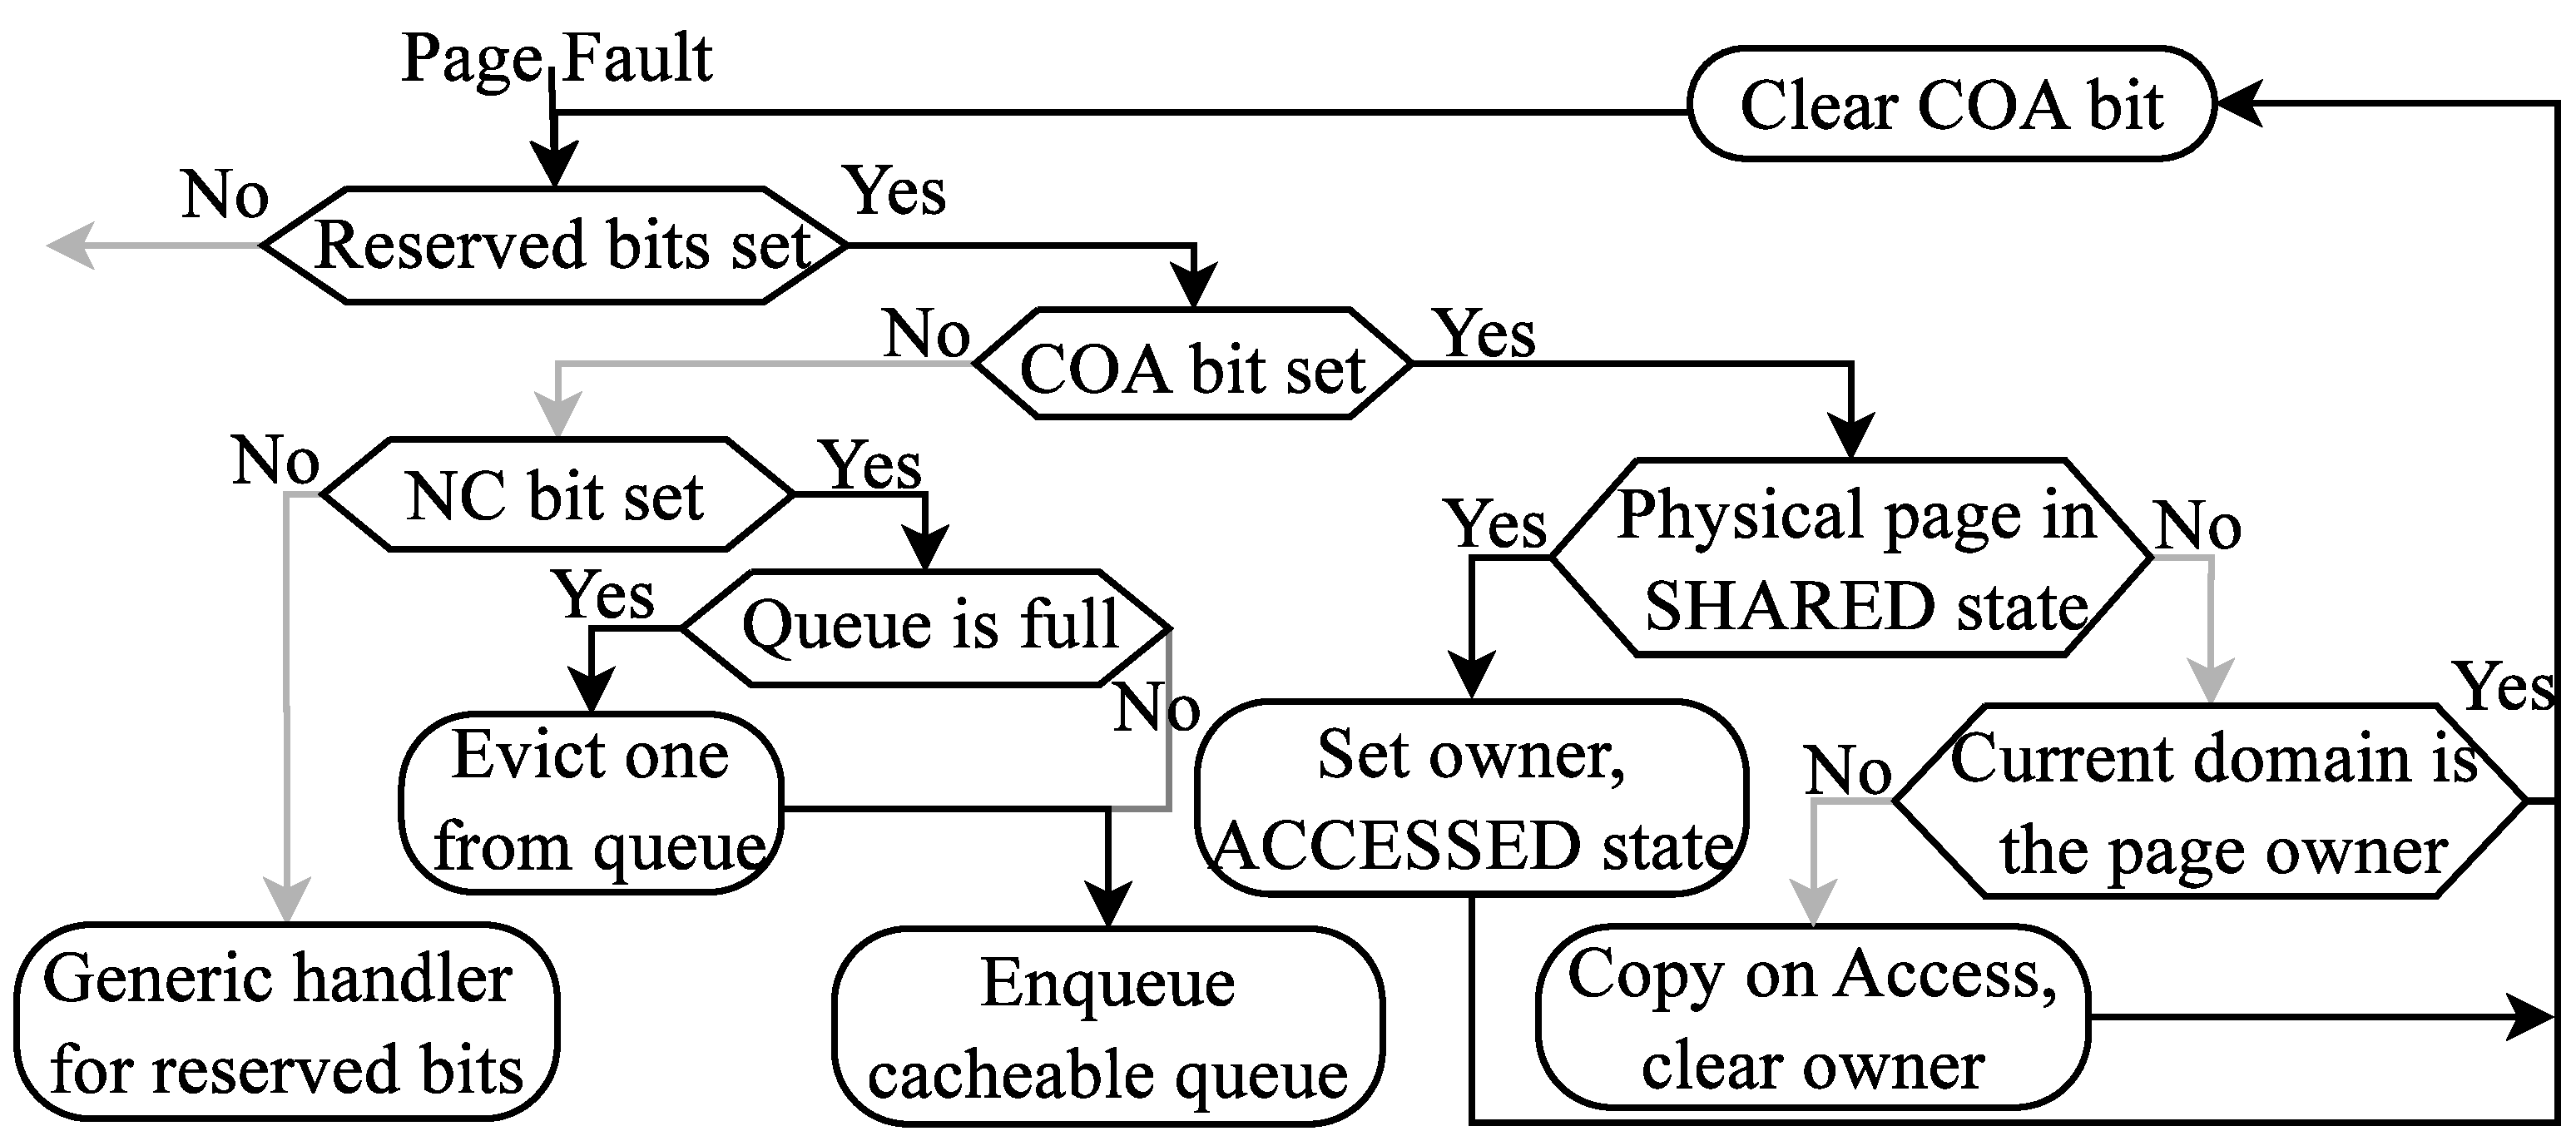
\includegraphics[width=0.9\linewidth]{fig/cachebar/page_fault.eps}
\caption{Page fault handler for \cachebar.\label{fig:fault}}
 \vspace{-0.1in}
\end{figure}

\bheading{Interacting with copy-on-access} The \lru{s} work closely
with the copy-on-access mechanisms. In particular, as both the \COA
and \LRU bits may trigger a page fault upon page accesses, the page
handler logic must incorporate both (see \figref{fig:fault}). First, a page
fault is handled as normal unless it is due to one of the reserved
bits set in the \gls{PTE}. As \cachebar is the only source of reserved bits,
it takes over page fault handling from this point. \cachebar first
checks the \COA bit in the \gls{PTE}. If it is set, the corresponding
physical page is either \shared, in which case it will be transitioned
to \accessed, or \accessed, in which case it will be copied and transitioned to either \shared or \exclusive.  \cachebar
then clears the \COA bit and, if no other reserved bits are set, the
fault handler returns.  Otherwise, if the \LRU bit is set, the
associated physical page is not in the \lru for its domain, and so
\cachebar enqueues the page and, if the queue is full, removes the
least-recently-used page from the queue.  If the \LRU bit is clear,
this page fault is caused by unknown reasons and \cachebar turns
control over to the generic handler for reserved bits.

\section{Security Evaluation}
\label{cachebar:sec:eval:security}
In this section, We empirically evaluated the effectiveness of \cachebar in
defending against both \flushreload and \primeprobe attacks.

Our testbed is a rack mounted DELL server equipped with two 2.67\gigahertz Intel Xeon
5550 processors. Each processor contains 4 physical cores (hyperthreading
disabled) sharing an 8\megabytes last-level cache (L3). Each core has a
32\kilobytes L1 data and instruction cache and a 256\kilobytes L2 unified cache.  The
rack server is equipped with 128\gigabytes DRAM and 1000\megabytes NIC connected to a
1000\megabytes ethernet.

We implemented \cachebar as a kernel extension for Linux kernel
3.13.11.6 that runs Ubuntu 14.04 server edition. We set up containers
using \docker 1.7.1.
\subsection{\flushreload attacks}
\label{cachebar:sec:eval:security:flushreload}
We
constructed a \flushreload covert channel between sender and
receiver processes, which were isolated in different containers. Both
the sender and receiver were linked to a shared library,
\texttt{libcrypto.so.1.0.0}, and were pinned to run on different cores
of the same socket, thus sharing the same last-level cache. The sender
ran in a loop, repeatedly accessing one memory location (the beginning
address of function \texttt{AES\_decrypt()}). The receiver executed
\flushreload attacks on the same memory address, by first \Flush{ing}
the memory block out of the shared \gls{LLC} with an \clflush instruction
and then \Reload{ing} the block by accessing it directly
while measuring the access latency. The interval between \Flush and
\Reload was set to 2500 \cycles. The experiment was run for 500,000
\flushreload trials.  We then repeated this experiment with the sender
accessing an unshared address, to form a baseline.

\begin{figure}[t]
\centering
\begin{subfigure}[b]{0.49\textwidth}
\includegraphics[width=0.95\linewidth]{fig/cachebar/eval/flushreload.eps}
\caption{\cachebar disabled}
\label{fig:flushreload_covert:linux}
\end{subfigure}
\begin{subfigure}[b]{0.49\textwidth}
\includegraphics[width=0.95\linewidth]{fig/cachebar/eval/flushreload-w.eps}
\caption{\cachebar enabled}
\label{fig:flushreload_covert:cachebar}
\end{subfigure}
\vspace{-0.1in}\caption{\Reload timings in \flushreload attacks on a
  shared address vs.\ on an unshared address}
\label{fig:flushreload_covert}
\end{figure}

\figref{fig:flushreload_covert:linux} shows the results of this
experiment, when run over unmodified Linux.
The three horizontal lines forming the ``box'' in each boxplot
represents the first, second (median), and third quartiles of the
\flushreload measurements; whiskers extend to cover all points that
lie within $1.5\times$ the interquartile range.  As can be seen in
this figure, the times observed by the receiver to \Reload the shared
address were clearly separable from the times to \Reload the unshared
address, over unmodified Linux.  With \cachebar enabled, however, these
measurements are no longer separable (\figref{fig:flushreload_covert:cachebar}).
Certain corner cases are not represented in
\figref{fig:flushreload_covert}.  For example, we found it extremely
difficult to conduct experiments to capture the corner cases where
\Flush and \Reload takes place right before and after physical page
mergers, as described in \secref{cachebar:sec:coa:security}. As such, we rely
on our manual inspection of the implementation in these cases to check
correctness and argue these corner cases are very difficult to exploit
in practice.

\subsubsection{Model Checking Noninterference}

%Model checking notation
\newcommand{\mcPagesArray}{\texttt{pages}\xspace}
\newcommand{\mcPages}[1]{\texttt{pages[{#1}]}\xspace}
\newcommand{\mcVirt}{\texttt{virt}\xspace}
\newcommand{\mcState}{\texttt{state}\xspace}
\newcommand{\mcOwner}{\texttt{owner}\xspace}
\newcommand{\mcNoOwner}{\texttt{none}\xspace}

\label{cachebar:sec:coa:security}
Copy-on-access is intuitively secure by design, as no two security
domains may access the same physical page at the same time, rendering
a general \Flush+\Reload attack seemingly impossible, as demonstrated in
previous section.  To show security formally, we subjected our design
to model checking in order to ensure that \coa is secure against
\flushreload attacks at every execution point.  Model checking is an
approach to formally verify a specification of a finite-state
concurrent system expressed as temporal logic formulas, by traversing
the finite-state machine defined by the model.  In our study, we used
the \spin model checker, which offers efficient ways to model
concurrent systems and verify temporal logic specifications.

\bheading{System modeling}
We model a physical page in \figref{fig:coa} using a byte
variable in the \textsc{Promela} programming language, and two
physical pages as an array of two such variables, named
\texttt{pages}.  We model two security domains (e.g., containers), an
attacker domain and a victim domain, as two processes in
\textsc{Promela}.  Each process maps a virtual page, \mcVirt, to one
of the physical pages. The virtual page is modeled as an index to the
\mcPagesArray{} array; initially \mcVirt for both the attacker and the
victim point to the first physical page (i.e., \mcVirt is $0$).  The
victim process repeatedly sets \mcPages{\mcVirt} to $1$, simulating a
memory access that brings \mcPages{\mcVirt} into cache.  The attacker
process \Flush{es} the virtual page by assigning $0$ to
\mcPages{\mcVirt} and \Reload{s} it by assigning $1$ to
\mcPages{\mcVirt} after testing if it already equals to $1$.  Both the
\Flush and \Reload operations are modeled as atomic to
simplify the state exploration.

We track the state and owner of the first physical page using another
two variables, \mcState and \mcOwner.  The first page is initially in
the \shared state (\mcState is \shared), and state transitions in
\figref{fig:coa} are implemented by each process when they access
the memory.  For example, the \Reload code snippet run by the attacker
is shown in \figref{fig:codesnippet}.  If the attacker has access to
the shared page (\lineref{lst:codesnippet:sharedPage}), versus an
exclusive copy (\lineref{lst:codesnippet:exclusivePage}), then it
simulates an access to the page, which either moves the state of the
page to \accessed (\lineref{lst:codesnippet:toAccessed}) if the state
was \shared (\lineref{lst:codesnippet:testShared}) or to \exclusive
(\lineref{lst:codesnippet:toExclusive}) after making a copy
(\lineref{lst:codesnippet:coa}) if the state was already \accessed and
not owned by the attacker (\lineref{lst:codesnippet:testAccessed}).
Leakage is detected if \mcPages{\mcVirt} is $1$ prior to the
attacker setting it as such (\lineref{lst:codesnippet:retrieve}), which
the attacker tests in \lineref{lst:codesnippet:leakage}.

\begin{figure}[h]
\vspace{-0.1in}
\lstset{language=Promela,
backgroundcolor=\color{white},
commentstyle=\scriptsize\ttfamily,
keepspaces=true,
basicstyle=\scriptsize\ttfamily,
keywordstyle=\scriptsize\bf,
numberstyle=\tiny\color{black},
rulecolor=\color{black},
morekeywords={atomic,if}
numbersep=8pt,
xleftmargin=2em,
breaklines=true, showstringspaces=false,
escapeinside={(*}{*)},
escapechar=|,
numberblanklines=false,
frame=lines, numbers=left, stepnumber=1} 
\centering
\begin{minipage}{0.7\linewidth}
\begin{lstlisting}
atomic {
if
::(virt == 0)|$\rightarrow$||\label{lst:codesnippet:sharedPage}|
   if
   ::(state == UNMAPPED) |$\rightarrow$||\label{lst:codesnippet:testUnmapped}|
      assert(0)
   ::(state == EXCLUSIVE && owner != ATTACKER) |$\rightarrow$\label{lst:codesnippet:testExclusive}|
      assert(0)
   ::(state == SHARED) |$\rightarrow$\label{lst:codesnippet:testShared}|
      state = ACCESSED|\label{lst:codesnippet:toAccessed}|
      owner = ATTACKER|\label{lst:codesnippet:chngOwner}|
   ::(state == ACCESSED && owner != ATTACKER) |$\rightarrow$\label{lst:codesnippet:testAccessed}|
      virt = 1  /* copy-on-access */|\label{lst:codesnippet:coa}|
      state = EXCLUSIVE|\label{lst:codesnippet:toExclusive}|
   fi
::else |$\rightarrow$| skip |\label{lst:codesnippet:exclusivePage}|
fi
assert(pages[virt] == 0) |\label{lst:codesnippet:leakage}|
pages[virt] = 1 |\label{lst:codesnippet:retrieve}|
}
\end{lstlisting}
\end{minipage}
\vspace{-0.1in}
\caption{Code snippet for \Reload.}
\label{fig:codesnippet}
\end{figure}

To model the dashed lines in \figref{fig:coa}, we implemented
another process, called \textit{timer}, in \textsc{Promela} that
periodically transitions the physical page back to \shared state from
\accessed state, and periodically with a longer interval, merges the
two pages by changing the value of \mcVirt of each domain back to $0$,
\mcOwner to \mcNoOwner, and \mcState to \shared.

The security specification is stated as a noninterference property.
Specifically, as the attacker domain always \Flush{es} the memory
block (sets \mcPages{\mcVirt} to $0$) before \Reload{ing} it (setting
\mcPages{\mcVirt} to $1$), if the noninterference property holds,
then the attacker should always find \mcPages{\mcVirt} to be $0$ upon
\Reload{ing} the page.  The model checker checks for violation of this
property.

\bheading{Automated verification}  We checked the model using
\spin. Interestingly, our first checking attempt suggested that
the state transitions may leak information to a \flushreload
attacker. The leaks were caused by the \textit{timer} process that
periodically transitions the model to a \shared state. After
inspecting the design and implementation, we found that there were two
situations that may cause information leaks.  In the first case, when
the timer transitions the state machine to the \shared state from the
\accessed state, if the prior owner of the page was the victim and the
attacker reloaded the memory right after the transition, the attacker
may learn one bit of information. In the second case, when the
physical page was merged with its copy, if the owner of the page was
the victim before the page became \shared, the attacker may reload it
and again learn one bit of information.  Since in our implementation
of \cachebar, these two state transitions are triggered if the page (or
its copy) has not been accessed for a while (roughly \accessedTimeout
and \copyTimeout seconds, respectively), the information leakage
bandwidth due to each would be approximately $1/\accessedTimeout$ bits
per page per second or $1/\copyTimeout$ bits per page per second,
respectively.

We improved our \cachebar implementation to prevent this leakage by
enforcing \gls{LLC} flushes (as described in \secref{cachebar:sec:coa:impl}) upon
these two periodic state transitions.  We adapted our model
accordingly to reflect such changes by adding one more instruction to
assign \mcPages{0} to be $0$ right after the two
\textit{timer}-induced state transitions.  Model checking this refined
model revealed no further information leakage.

\subsection{\primeprobe attacks}
\label{cachebar:sec:eval:security:primeprobe}

We evaluated the effectiveness of \cachebar against \primeprobe attacks
by measuring its ability to interfere with a simulated attack.
Because the machine architecture on which we performed these tests had
a \cacheLineNmbr-way \gls{LLC} with $\cacheLineNmbr=16$, we limited our
experiments to only a single attacker container (i.e.,
$\attackerNmbr=1$), but an architecture with a larger \cacheLineNmbr
could accommodate more.\footnote{For example, on an Itanium 2
processor with a 64-way \gls{LLC}, \cachebar could accommodate $\attackerNmbr
= 3$ or larger.  That said, we are unaware of prior works that have
successfully conducted \primeprobe attacks from multiple colluding
attackers, which would itself face numerous challenges (e.g.,
coordinating \Probe{s} by multiple processes).}

In our simulation, a process in the attacker container repeatedly
performed \primeprobe attacks on a specific cache set, while a process
in a victim container accessed data that were retrieved into the same
cache set at the rate of $\victimDemand$ accesses per attacker
\primeprobe interval.  The cache lines available to the victim
container and attacker container, i.e.,
$\linesPerContainer{\victimLabel}$ and
$\linesPerContainer{\attackerLabel}$ respectively, were fixed in each
experiment.  The calculations in
\secref{cachebar:sec:cacheabilityMgmt:security} implied that
$\linesPerContainer{\victimLabel}$ and
$\linesPerContainer{\attackerLabel}$ could take on values from
$\{4,5,6,\ldots,14\}$.  In each test with fixed
\linesPerContainer{\victimLabel} and
\linesPerContainer{\attackerLabel}, we allowed the victim to place a
demand of (i.e., retrieve memory blocks to fill) $\victimDemand \in
\{0, 1, 2,...,16\}$ cache lines of the cache set undergoing the
\primeprobe attack by the attacker.  The attacker's goal was to
classify the victim's demand into one of six classes: $\classNone =
\{0\}$, $\classOne =\{1\}$, $\classFew=\{2,3,4\}$,
$\classSome=\{5,6,7,8\}$, $\classLots=\{9,10,11,12\}$, and
$\classMost=\{13,14,15,16\}$.

To make the attack easier, we permitted the attacker to
know \linesPerContainer{\attackerLabel}; i.e., the attacker trained a
different classifier per value of \linesPerContainer{\attackerLabel},
with knowledge of the demand \victimDemand per \primeprobe trial, and
then tested against additional trial results to classify unknown
victim demands.  Specifically, after training a \naive{} Bayes
classifier on 500,000
\primeprobe trials per $(\victimDemand,
\linesPerContainer{\attackerLabel}, \linesPerContainer{\victimLabel})$
triple, we tested it on another 500,000 trials. To filter out \Probe
readings due to page faults, excessively large readings were discarded
from our evaluation. The tests without \cachebar yielded
the confusion matrix in \tabref{fig:confusion:disabled}, with overall
accuracy of 67.5\%.  In this table, cells with higher numbers have
lighter backgrounds, and so the best attacker would be one who
achieves white cells along the diagonal and dark-gray cells elsewhere.
As can be seen there, classification by the attacker was very accurate
for \victimDemand falling into \classNone, \classOne, or \classLots;
e.g., $\victimDemand=1$ resulted in a classification of \classOne with
probability of $0.80$.  Other demands had lower accuracy, but
were almost always classified into adjacent classes; i.e.,
\textit{every} class of victim demand was classified correctly or as
an adjacent class (e.g., $\victimDemand \in \classFew$ was classified
as \classOne, \classFew, or \classSome) at least 96\% of the time.

\begin{figure}[tb]
\setlength\tabcolsep{1.5pt}
\ExplSyntaxOn
\fp_set:Nn \MinVal {0.0}
\fp_set:Nn \MaxVal {1.0}
\ExplSyntaxOff
\begin{center}
\begin{subfigure}[b]{0.495\textwidth}
\resizebox{\textwidth}{!}{
{\footnotesize
      \begin{tabular}{@{\hspace{0pt}}crRRRRRR}
       &  & \multicolumn{6}{c}{Classification by attacker} \\
       &  & \multicolumn{1}{c}{\classNone}& \multicolumn{1}{c}{\classOne}&
	   \multicolumn{1}{c}{\classFew}& \multicolumn{1}{c}{\classSome}&
	   \multicolumn{1}{c}{\classLots}&
	   \multicolumn{1}{c}{\classMost}\\\cline{3-8}\\[-2.8ex]
        \multirow{6}{*}{\rotatebox[origin=c]{90}{{\centering Victim demand \victimDemand}}} 
       &  \multicolumn{1}{r|}{\classNone}& .96& .04& .00& .00& .00& .00 \\
       & \multicolumn{1}{r|}{\classOne}& .01& .80& .19& .01& .00& .00 \\
       &  \multicolumn{1}{r|}{\classFew}& .00& .16& .50& .30& .04& .00 \\
       &  \multicolumn{1}{r|}{\classSome}& .00& .00& .07& .54& .34& .04 \\
       &  \multicolumn{1}{r|}{\classLots}& .00& .00& .00& .03& .84& .13 \\
       &  \multicolumn{1}{r|}{\classMost}& .00& .00& .00& .03& .56& .41 \\
        \multicolumn{7}{c}{~} \\
      \end{tabular}
      }
}
\caption{Without \cachebar\label{fig:confusion:disabled}}
\end{subfigure}
\begin{subfigure}[b]{0.495\textwidth}
\resizebox{\textwidth}{!}{
{\footnotesize
	\begin{tabular}{@{\hspace{0pt}}crRRRRRR}
	&  & \multicolumn{6}{c}{Classification by attacker} \\
		&  & \multicolumn{1}{c}{\classNone}& \multicolumn{1}{c}{\classOne}&
		\multicolumn{1}{c}{\classFew}& \multicolumn{1}{c}{\classSome}&
		\multicolumn{1}{c}{\classLots}&
		\multicolumn{1}{c}{\classMost}\\\cline{3-8}\\[-2.8ex]
		\multirow{6}{*}{\rotatebox[origin=c]{90}{{\centering Victim demand \victimDemand}}} 
	& \multicolumn{1}{r|}{\classNone}& .33& .16& .26& .18& .04& .02 \\
		& \multicolumn{1}{r|}{\classOne}& .16& .36& .19& .19& .06& .04 \\
		& \multicolumn{1}{r|}{\classFew}& .13& .14& .40& .19& .09& .05 \\
		& \multicolumn{1}{r|}{\classSome}& .09& .10& .16& .37& .20& .07 \\
		& \multicolumn{1}{r|}{\classLots}& .08& .06& .10& .16& .46& .13 \\
		& \multicolumn{1}{r|}{\classMost}& .10& .07& .18& .18& .18& .29 \\
		\multicolumn{8}{c}{~} \\
		\end{tabular}
}
}
\caption{With \cachebar \label{fig:confusion:enabled}}
\end{subfigure}
\end{center}
\vspace{-0.2in}
\caption{Confusion matrix of \naive{} Bayes classifier}
\label{fig:confusion}
\end{figure}


In contrast, \figref{fig:confusion:enabled} shows the confusion matrix
for a \naive{} Bayes classifier trained and tested using \primeprobe
trials conducted with \cachebar enabled.  Specifically, these values
were calculated using
\begin{align*}
\cprob{\big}{}{\classifiedRV = \classId}{\victimDemand\in\classIdAlt} 
= \sum_{4 \le \attackerLineNmbr, \victimLineNmbr \le 14}
  \left(\begin{array}{r}
    \cprob{\Big}{}{\classifiedRV\!=\!\classId\!}{\!\victimDemand\in\classIdAlt \wedge \victimLineNmbrRV = \victimLineNmbr
  \wedge~\attackerLineNmbrRV\!=\!\attackerLineNmbr} \\
  \cdot~\prob{}{\attackerLineNmbrRV\!=\!\attackerLineNmbr}
  \cdot \prob{}{\victimLineNmbrRV\!=\!\victimLineNmbr}
  \end{array}\right)
\end{align*}
where \classifiedRV denotes the classification obtained by the
adversary using the \naive{} Bayes classifier; $\classId, \classIdAlt \in
\{\classNone$, \classOne, \classFew, \classSome, \classLots,
$\classMost\}$; and $\prob{}{\attackerLineNmbrRV = \attackerLineNmbr}$
and $\prob{}{\victimLineNmbrRV = \victimLineNmbr}$ are calculated as
described in \secref{cachebar:sec:cacheabilityMgmt:security}.  The factor\\
$\cprob{\big}{}{\classifiedRV=\classId}{\victimDemand\in\classIdAlt
  \wedge \victimLineNmbrRV = \victimLineNmbr \wedge
  \attackerLineNmbrRV = \attackerLineNmbr}$ was measured empirically.
Though space limits preclude reporting the full class confusion matrix
for each \victimLineNmbr, \attackerLineNmbr pair, the accuracy of the
\naive{} Bayes classifier per \victimLineNmbr, \attackerLineNmbr pair,
averaged over all classes \classId, is shown in \figref{fig:accuracy}.
As in \figref{fig:confusion}, cells with larger values in
\figref{fig:accuracy} are more lightly colored, though in this case,
the diagonal has no particular significance. The design intuitively
assumes when the attacker and victim are each limited to fewer lines
in the cache set (i.e., small values of \attackerLineNmbr and
\victimLineNmbr, in the upper left-hand corner of
\figref{fig:accuracy}) the accuracy of the attacker will suffer,
whereas when the attacker and victim are permitted to use more lines
of the cache (i.e., in the lower right-hand corner) the attacker's
accuracy would improve.  \figref{fig:accuracy} supports these general
trends.

\begin{figure}[t]
\begin{center}
\ExplSyntaxOn
\fp_set:Nn \MinVal {0.17}
\fp_set:Nn \MaxVal {0.68}
\ExplSyntaxOff
{\fontsize{10pt}{11pt}\selectfont
\begin{tabular}{@{\hspace{0pt}}c@{\hspace{0.5em}}r|TTTTTTTTTTT}
& \multicolumn{1}{r}{~} & \multicolumn{11}{c}{\small{$\linesPerContainer{\victimLabel}$}} \\
& \multicolumn{1}{r}{~} & \multicolumn{1}{c}{4}& \multicolumn{1}{c}{5}& \multicolumn{1}{c}{6}& \multicolumn{1}{c}{7}& \multicolumn{1}{c}{8}& \multicolumn{1}{c}{9}& \multicolumn{1}{c}{10}& \multicolumn{1}{c}{11}& \multicolumn{1}{c}{12}& \multicolumn{1}{c}{13}& \multicolumn{1}{c}{14} \\\cline{3-13}\\[-2.485ex]
\parbox[t]{1mm}{\multirow{11}{*}{\rotatebox[origin=c]{90}{\small{$\linesPerContainer{\attackerLabel}$}}}} 
& 4 & .18& .17& .17& .17& .17& .17& .17& .17& .36& .22& .33 \\
& 5 & .19& .17& .30& .32& .27& .27& .20& .26& .33& .46& .39 \\
& 6 & .17& .31& .24& .18& .21& .17& .20& .27& .43& .39& .41 \\
& 7 & .17& .33& .22& .22& .19& .31& .33& .33& .46& .48& .54 \\
& 8 & .33& .35& .32& .23& .43& .37& .43& .42& .32& .38& .49 \\
& 9 & .20& .26& .31& .28& .44& .38& .34& .34& .46& .39& .56 \\
& 10& .41& .31& .27& .35& .50& .55& .53& .31& .53& .50& .62 \\
& 11& .45& .45& .40& .45& .47& .54& .54& .57& .67& .50& .50 \\
& 12& .55& .50& .59& .63& .49& .48& .54& .49& .56& .58& .57 \\
& 13& .55& .53& .68& .68& .54& .65& .52& .56& .57& .66& .66 \\
& 14& .53& .56& .45& .65& .46& .62& .48& .68& .55& .57& .53 \\
\end{tabular}
}
\end{center}
\vspace{-0.1in}
\caption{Accuracy per values of \victimLineNmbr and \attackerLineNmbr}
\label{fig:accuracy}
\end{figure}

\figref{fig:confusion:enabled} shows that \cachebar
substantially degrades the adversary's classification accuracy, which
overall is only 33\%.  Moreover, the adversary is not only
wrong more often, but is also often ``more wrong'' in those cases.
That is, whereas in \figref{fig:confusion:disabled} shows that each
class of victim demand was classified as that demand or an adjacent
demand at least 96\% of the time, this property no longer holds true
in \figref{fig:confusion:enabled}.  Indeed, the attacker's
\textit{best} case in this regard is classifying victim demand
\classLots, which it classifies as \classSome, \classLots, or
\classMost 75\% of the time.  In the case of a victim demand of
\classMost, this number is only 47\%.


\section{Summary}
This chapter presented two techniques to defend against side-channel
attacks via \glspl{LLC}, namely (i) copy-on-access for physical pages shared
among multiple security domains, to interfere with \flushreload
attacks, and (ii) cacheability management for pages to limit the
number of cache lines per cache set that an adversary can occupy
simultaneously, to mitigate \primeprobe attacks.  Using formal
analysis (model checking for copy-on-access, and probabilistic
modeling for cacheability management), we developed designs that
mitigate side-channel attacks in our empirical evaluations. We also
learned a lesson that the experiment-based leakage measure covers
fewer leaks than a static analysis because its empirical data is
limited to concrete attacks.  
